%%%%%%%%%%%%%%%%%%%%%%%%%%%%%%%%%%%%%%%%%%%%%%%%%%%%%%%%%%%%%%%%%%%%%%%%%%%%%%%%
\begin{abstract}

	\textbf{Calculating music similarity metrics using map reduce algorithms.}\\
	This paper is about the comparison of construction noise and modern day music. 
	The field of music information retrieval (MIR) in computer science is mostly a data driven and purely mathematical topic. The goal of this paper is to merge the fields of computer science with music theoretical knowledge and to find potential weak spots of current music similarity algorithms. 

\end{abstract}

%----------------------------------------------------------------------------------------
%	THESIS CONTENT - CHAPTERS
%----------------------------------------------------------------------------------------

\mainmatter % Begin numeric (1,2,3...) page numbering
\pagenumbering{arabic}

%%%%%%%%%%%%%%%%%%%%%%%%%%%%%%%%%%%%%%%%%%%%%%%%%%%%%%%%%%%%%%%%%%%%%%%%%%%%%%%%
\chapter{Introduction}

The idea originated from Dr. T. Bosse from the chair for advanced computing at the Friedrich-Schiller-University (FSU) in Jena. When proposing the idea for a master thesis with the topic of "Music similarity measurement using genre specific features" using different guitar play styles in modern day metal music, he jokingly said that he would also like to know how metal music compares to construction building noise.
The idea is actually not so groundless, considering that most people would agree on the fact that metal music is often described as noise by people not used to listening to genres like death and black metal.
This thesis is meant to evaluate how music similarity algorithms compare construction noise to common musical genres and how to possibly improve these algorithms.

\section{Why and how?}

\underline{Why is music similarity research even necessary?} 
\ \\
\ \\
First of all, there is no fixed definition of music similarity so far. This is one of the first problems, dealing with music similarity. This topic offers multifaceted approaches. Merging multiple approaches with different weights can offer a more diverse music recommendation system. To do this, a lot of different data is required.\\
Content (music features) and context (listener behaviour) data can be fed into a big data framework to speed up operations.
Collecting this data for large amounts of songs results in big datasets that need to be explored efficiently.\\
\ \\
\underline{What to improve?}
\ \\
\ \\
"[...] Spotify Radio, iTunes Radio, Google Play Access All Areas and Xbox Music. Recommendations are typically made using (undisclosed) content-based retrieval techniques, collaborative filtering data or a combination thereof." \cite[p. 9]{knees1}
The goal of this work is, to propose a transparent music similarity retrieval method based on various weighted contextual and content-based data. 
Applying different weights to different features allows similarity retrieval methods to search for different kind of similarity. 
E.g. weighing the tempo and beat of a song more then melodic similarity allows the creation of playlists for workout and sport, whilst melodic/ timbre etc. similarities allows to search for similar songs from musical subgenres. 
The user would get to decide what kind of playlist he wants to create. 
Adding contextual data and feeding it to an algorithm could add more or less popular music to the playlist with the goal to discover new upcoming artists or get other popular and most listened music. 
For this thesis however, the focus lies on content-based data/ audio features.\\ 
\ \\
\underline{How to approach this?}
\ \\
\ \\
First of all, a lot of data is required. In the first part, different scientific datasets are evaluated. 
Secondly, the available features are shown and explained. 
In the third part, different metrics are explained using the previously explored features. 
Lastly, a big data approach to efficiently use the gathered features is proposed and evaluated. A way to evaluate the results is also proposed.

\section{Overview}

\textit{Structure: \\}
\ \\
\smartdiagramset{set color list={blue!40!white, blue!40!white,blue!40!white, blue!40!white, blue!40!white}}
\tikzset{priority arrow/.append style={rotate=180,anchor=0,xshift=30,}}
\smartdiagram[priority descriptive diagram]{PART IV: Performance Tuning, PART III: Similarity Estimation, PART II: Feature Extraction, PART I: Data Aggregation}


\chapter{MIR Toolkits and audio features}

\section{Music Information Retrieval}
The field of music information retrieval is a large research area combining studies in computer science like signal processing and machine learning as well as psychology and academic music study.
The algorithm used in this paper is described in \cite[pp. 17ff]{schnitzer1} and in section \ref{mfccsim}.
The framework used to determine the song similarity in chapter \ref{musly} is the MUSLY toolkit \cite{musly1}
To get started, a brief overview is given in the next section providing the most important information about publicly available datasets, MIR toolkits and approaches to music similarity.

\section{Audio Features and Music Similarity Measurements}

This section provides an overview about different music similarity measurements and metrics.\\
More in-depth information about the different metrics is given in chapter \ref{simmet}

\subsection{Frequency based}\label{featsec}

As done by: \cite[pp. 17ff]{schnitzer1}\\
Most of the algorithms start with switching from the time domain to the frequency domain, by performing a Discrete Fourier transform as described in equation \ref{eq:fft} and then compute the power spectrum (equation \ref{eq:absfft})

\begin{equation} \label{eq:fft}
%p (v \vert \lambda)=\sum_{i=1}^{M}w_iN(v \vert \mu_i,\sum_i) \label{prob}
X_m = \sum_{k=0}^{K-1}{x_k \cdot e^ { - \frac{K}{ 2 \cdot \pi \cdot i}\cdot k\cdot m}}
\end{equation}

\begin{equation} \label{eq:absfft}
%p (v \vert \lambda)=\sum_{i=1}^{M}w_iN(v \vert \mu_i,\sum_i) \label{prob}
|X_m| = \sqrt{Re(X_m)^2 + Im(X_m)^2}
\end{equation}

Figure \ref{laylaspec} shows the spectrogram of the first bars of the song Layla by Eric Clapton. The sound sample was recorded on an electric guitar to avoid copyright infringements. 
Due to the fact that the human ear perceives sound in a non-linear matter, a logarithmic or Mel-scale is better to represent different pitches.\\ 
For example the note A4 is perceived at a frequency of 440Hz, the A note of next octave (A5) is at 880Hz and the next one is at 1600Hz and so on. 
The Mel-scale \cite[pp. 53f]{knees1} was introduced to resemble the human perception of frequency (equation \ref{eq:mel})

\begin{equation} \label{eq:mel}
%p (v \vert \lambda)=\sum_{i=1}^{M}w_iN(v \vert \mu_i,\sum_i) \label{prob}
m = 1127 \cdot ln(1 + \frac{f}{700})
\end{equation}

The following plots were created with the librosa library \cite{librosa1}.

\begin{figure}[htbp]
	\centering
	\begin{subfigure}{0.5\textwidth}
		\centering
		\framebox{\parbox{2.96in}{      
		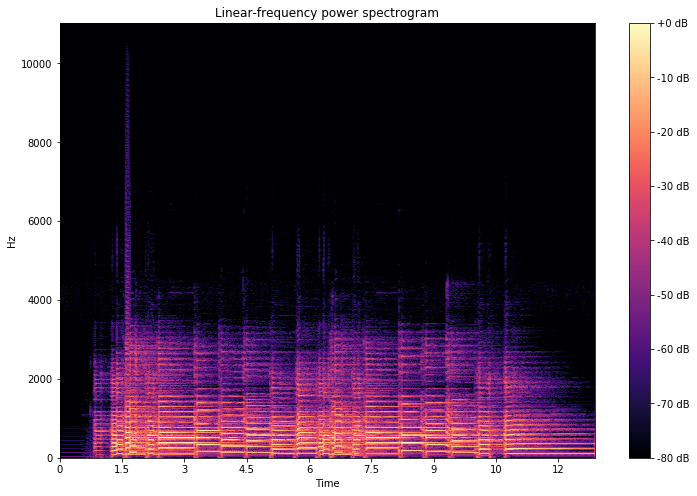
\includegraphics[scale=0.25]{Images/Layla/laylacfft.png}}}
		\captionof{figure}{Spectrogram}
		\label{laylaspec}
	\end{subfigure}%
	\begin{subfigure}{0.5\textwidth}
		\centering
		\framebox{\parbox{2.96in}{      
		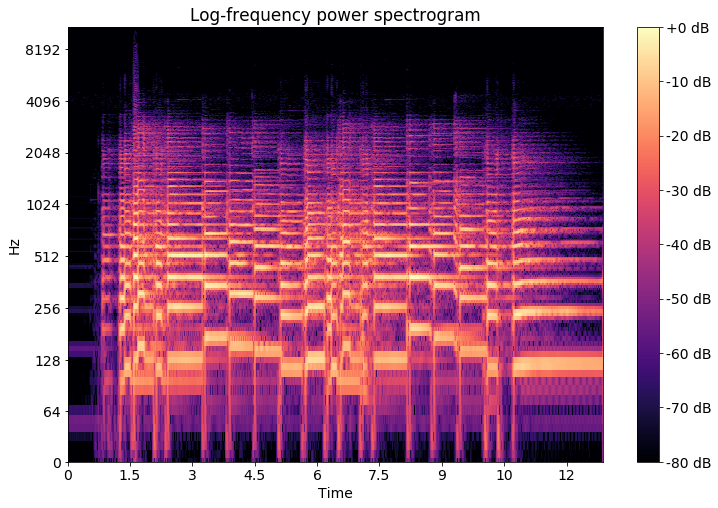
\includegraphics[scale=0.25]{Images/Layla/laylacfftlog.png}}}
		\captionof{figure}{Rachmaninoff Prelude in C Sharp Minor \cite{rm1}}
		\label{laylaspecfft}
	\end{subfigure}
	\caption{Frequency Space}
	\label{fig:test}
\end{figure}

The high dimensionality of the data is a problem for machine learning applications and music similarity tasks, as computation based on a vector with such a high dimensionality of the data would take to long.
Given a sample rate of $f_s = 44,1kHz$ (usual CD sample-rate) and a length of a song of about $t = 180s$, the time domain contains 7938000 data points usually with 16-bit resolution. 

\begin{equation} \label{eq:points}
%p (v \vert \lambda)=\sum_{i=1}^{M}w_iN(v \vert \mu_i,\sum_i) \label{prob}
K = f_s \cdot t
\end{equation}

Calculating a FFT with a window size of 1024 samples and a hop size of 512 samples (resulting in the factor 1.5 in equation \ref{eq:hop})\cite{knees1}, the full resulting spectrogram would contain 11627 frames with 1024 frequency values per frame. (eq: \ref{eq:hop}) 

\begin{equation} \label{eq:hop}
%p (v \vert \lambda)=\sum_{i=1}^{M}w_iN(v \vert \mu_i,\sum_i) \label{prob}
N_{fv} = 1.5 \cdot (\frac{44100 \ samples/s}{1024 \ samples/frame}) \cdot t
\end{equation}

To reduce the dimensionality of the feature vector, a typical approach in MIR would be to calculate the so called Mel Frequency Cepstral Coefficients (MFCCs). They are described in more detail in the next section.

\begin{figure}[htbp]
	\centering
	\framebox{\parbox{1\textwidth}{ 
			\begin{subfigure}{.495\textwidth}
				\centering 
				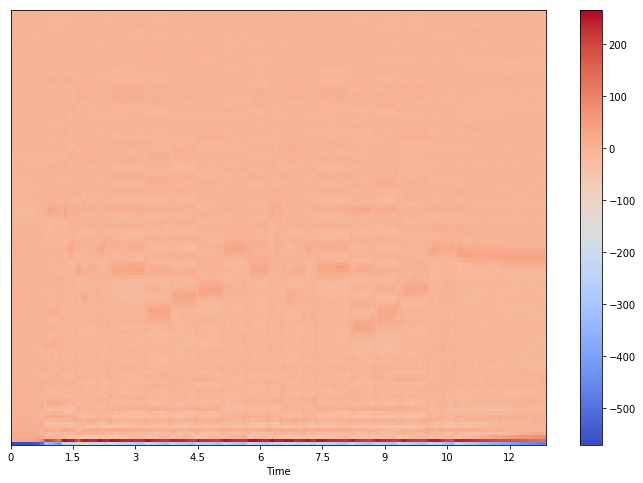
\includegraphics[scale=0.3]{Images/Layla/laylacmfccHR.png}
				\caption{MFCC High Resolution}
				\label{laylacmfcchr}
			\end{subfigure}%
			\begin{subfigure}{.495\textwidth}
				\centering
				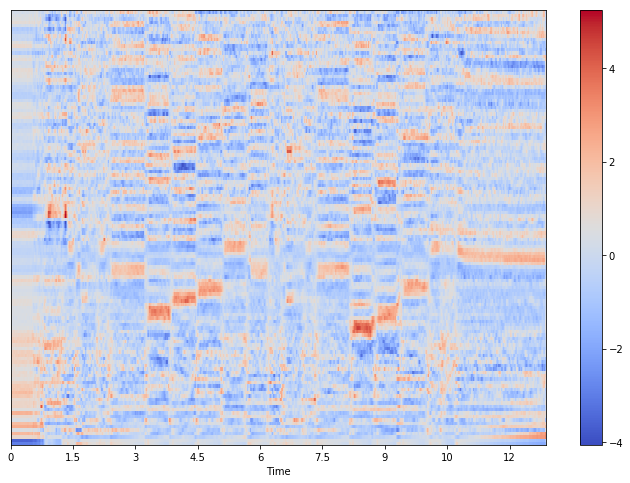
\includegraphics[scale=0.3]{Images/Layla/laylacmfccscaled.png}
				\caption{MFCC High Resolution Scaled}
				\label{laylacmfccscaled}
			\end{subfigure}%
	}}
	\caption{Features}
	\label{fig:feat1}
\end{figure}

As another, better comprehensible feature set, the chroma features represent the tonal properties of a song. The chroma plot (Figure \ref{laylachroma}) shows the distribution of the different pitches mapped to the various keys in one octave. The values are normalized to one by the strongest dimension. So if all values are close to one, it is most likely that there is only noise at that frame in the recording, as depicted in the first frames of figure \ref{laylachroma}.
Figure \ref{laylapitch} figures the pitch curve of the recording. None but the most dominant frequencies are shown. Pitches below a certain threshold are filtered out. These Pitch curves can be used to estimate and transcribe musical notes from audio data as presented in \ref{midiest}. 
The Plot in figure \ref{laylacbeat} shows the onsets (beginning of musical notes) and estimated beats.
%In the last picture the chroma plot is cleaned up, filtered for the most dominant pitches and pictured alongside the detected beats. 

\begin{figure}[htbp]
	\centering
	\framebox{\parbox{1\textwidth}{ 
			\begin{subfigure}{.495\textwidth}
				\centering 
				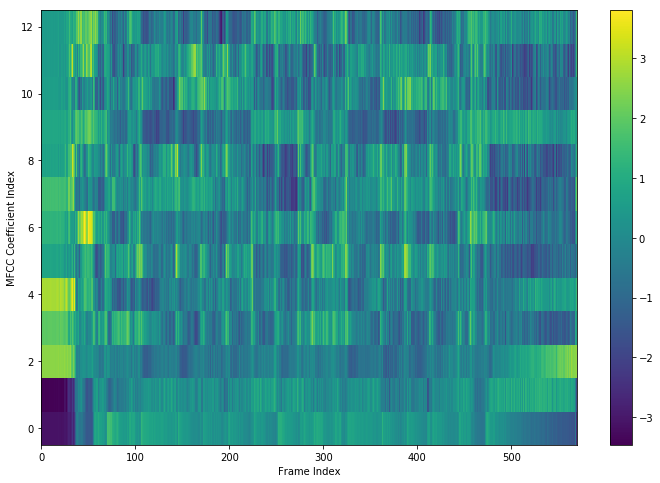
\includegraphics[scale=0.3]{Images/Layla/laylacmfcc.png}
				\caption{MFCC}
				\label{laylacmfcc}
			\end{subfigure}%
			\begin{subfigure}{.495\textwidth}
				\centering    
				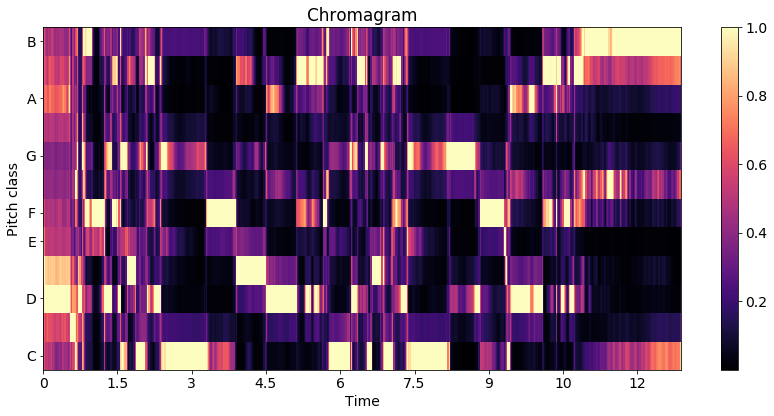
\includegraphics[scale=0.3]{Images/Layla/laylachroma.png}
				\caption{Chroma Features}
				\label{laylachroma}
			\end{subfigure}%
			
			\begin{subfigure}{.495\textwidth}
				\centering
				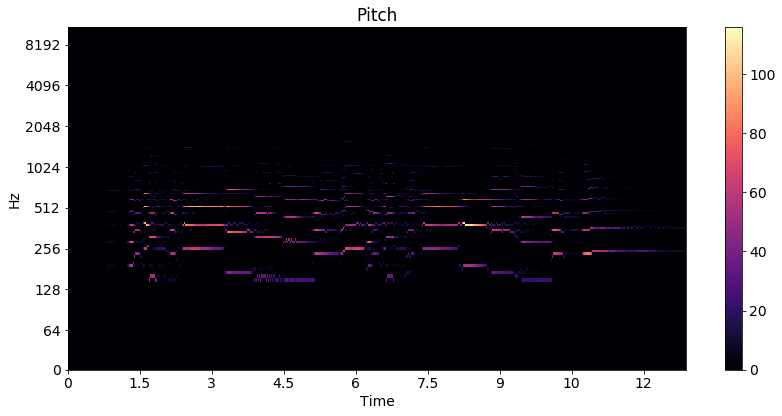
\includegraphics[scale=0.3]{Images/Layla/laylapitch.png}
				\caption{Pitch}
				\label{laylapitch}
			\end{subfigure}%
			\begin{subfigure}{.495\textwidth}
				\centering     
				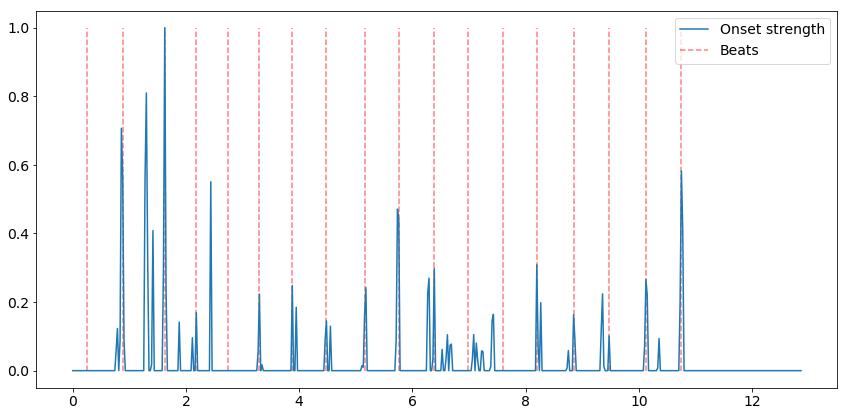
\includegraphics[scale=0.3]{Images/Layla/laylabeat.png}
				\caption{Rhythm/ Beat}
				\label{laylacbeat}
			\end{subfigure}%
	}}
	\caption{Features}
	\label{fig:feat2}
\end{figure}

\subsection{MFCC}\label{mfccsim}

This section gives a brief overview over the computation of the MFCC as stated in \cite[pp. 55ff]{knees1}.
Figure \ref{sweep} shows the magnitude spectrum of a frequency sweep signal.

\begin{figure}[htbp]
	\centering
	\framebox{\parbox{1\textwidth}{ 
	\begin{subfigure}{.495\textwidth}
		\centering 
		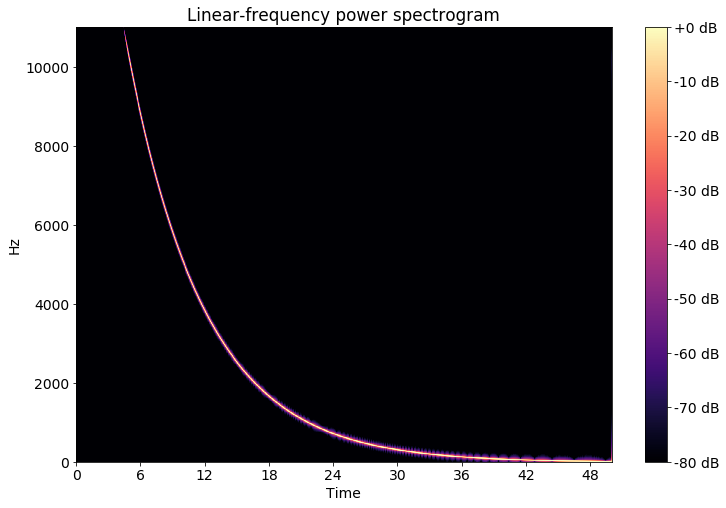
\includegraphics[scale=0.25]{Images/MFCC/sweep.png}
		\caption{Sweep signal linear}
		\label{sweeplog}
	\end{subfigure}
	\begin{subfigure}{.495\textwidth}
		\centering
		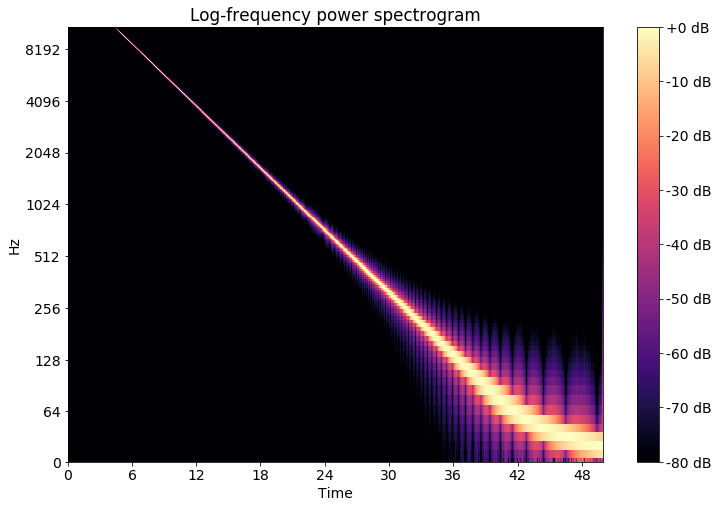
\includegraphics[scale=0.25]{Images/MFCC/sweeplog.png}
		\caption{Sweep signal logarithmic}
		\label{sweeplin}
	\end{subfigure}
	}}
	\caption{Sweep Sinal}	
	\label{sweep}
\end{figure}
\FloatBarrier

First of all the magnitude spectrum is transformed to the Mel-scale by assigning each frequency value to a Mel- band.
Doing this a dimension reduction can be done, by assigning multiple frequency values to one of typically 12 to 40 Mel-bands. The resulting vectors are then fed into a discrete cosine transformation (DCT) resulting in the MFCCs for each frame. 

\begin{equation} \label{eq:dct}
%p (v \vert \lambda)=\sum_{i=1}^{M}w_iN(v \vert \mu_i,\sum_i) \label{prob}
X_k = \sum_{n=0}^{N-1}{x_n cos\left[{\frac{\pi}{N}(n + \frac{1}{2})k}\right]}
\end{equation}

Figure \ref{mfcc} shows the resulting MFCCs with a high resolution of 1024 Mel bands. This is not what in a usual application would be done, because this is nearly as high dimensional as the original spectrogram. Figure \ref{mfccs} shows the MFCC reduced to 12 Mel Bands.


\begin{figure}[htbp]
	\centering
	\framebox{\parbox{1\textwidth}{ 
	\begin{subfigure}{.495\textwidth}
		\centering 
		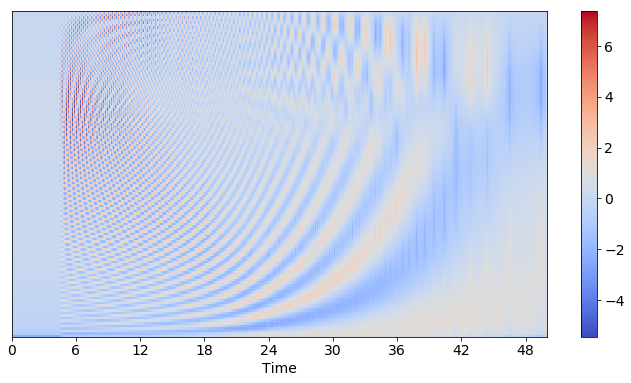
\includegraphics[scale=0.25]{Images/MFCC/mfccscaled.png}
		\caption{MFCC High Resolution}
		\label{mfcc}
	\end{subfigure}
	\begin{subfigure}{.495\textwidth}
		\centering
		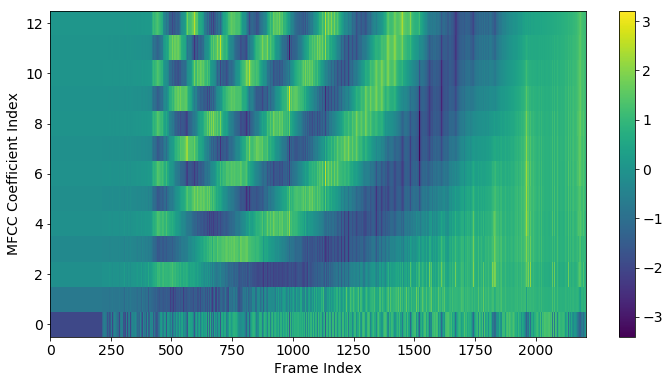
\includegraphics[scale=0.25]{Images/MFCC/mfccnorm.png}
		\caption{MFCC 12 Bands scaled}
		\label{mfccs}
	\end{subfigure}
	}}
	\caption{MFCCs}	
	\label{fig:mfcc}
\end{figure}
\FloatBarrier

\subsection{Rhythm based}
As done by: \cite{rhythm1}\\
Rhythm based music similarity algorithms use timing information of various events. The so called rhythm spectrum can be used as a feature vector.
For example the onset and beat data from the plot in Figure \ref{laylacbeat} could be used as a starting point for rhythmic similarity retrieval.
An in depth overview is given in chapter \ref{rhythmsimc}

\subsection{Pitch based}

As done by: \cite{pitch1}\\
The proposed approach by \cite{pitch1} is, to take mid-level features like chroma or pitch instead of high-level features like sheet music or low-level features like gaussian mixture models of MFCCs. 
A more detailed analysis of this topic is given in chapter \ref{melsimc}


\subsection{Metadata based/ Collaborative Filtering}

As done by: \cite{metadat1} and \cite{msd4} using the Million Song Dataset (MSD) \cite{msd1}\\
In 2012 the MSD Challenge was brought to the MIR community. The researches were challenged to give a list of song recommendations based on a large set of user data.\\ 
So if user X listened a lot to artist A and artist B and user Y listens mostly to artist A and artist C, then maybe user X would like artist C as well. 
These kind of metadata based recommendations are pretty common in large music streaming services, although not necessarily representing direct musical similarity.
These kind of recommendation systems tend to propose commonly well known artists rather than not so well known ones biasing the result. 
On the other hand these kind of similarity algorithms can work very fast and efficient.  

\subsection{Note based}

As done by: \cite{midi1}\\
For comparing musical pieces by their symbolic represenation (notes, tabulatures etc.) different text retrieval methods could be used. The MIDI datatype could be used, as it is a form of digital representation of music information. 
\cite{midi1} uses a variation of the Levinshtein distance measurement. 
The problem with notation based algorithms is, that there are not many datasets available containing audio and MIDI information.
As shown in \ref{midiest} the automatic transcription of notes from raw audio does not work flawlessly. 
There is ongoing research to automatically annotate musical notes with the help of neural networks.\cite{crepe1}

\subsection{Genre specific features}

As done by: \cite{mussim1} for indian art music, by using 560 different combinations of different features. They state that: "We evaluate all possible combinations of the choices made at each step of the melodic similarity computation discussed in Section 2.  We consider 5 different sampling rates of the melody representation, 8 different normalization scenarios, 2 possibilities of uniform time-scaling and 7 variants of the distance measures.  In total, we evaluate 560 different variants" \cite[p. 3]{mussim1}. This evaluation showed, that the choice of features and parameters for music similarity measurement is a critical point.\\
In Rock, Pop and Metal music, extraction of different guitar playstyles would be imaginable. Guitar Tab Extraction \cite{guitext1} Toolkits could be used to extract information if the guitar in a song is mostly plucked or strummed for instance. Or if there are Hammer-on/ Pull-off/ side bending or tapping techniques used.
In classical music, the play style of the string section of an orchestra could be taken into consideration. 

\section{MIR Toolkits}\label{mirtoolkit}
\subsection{Music Similarity}

The easiest way to test state of the art music similarity algorithms is to use the open source toolkit Musly \cite{musly1}\\ 
It is based on statistical models of MFCC features and calculates the distances between songs very fast, supporting OpenMP acceleration. It offers the classical mandel-ellis similarity method \cite{mandelellis1} and a timbre based improved version of the mandel-ellis algorithm \cite{musly2}\\
The MIR Toolkit \cite{mirtoolbox1} is a toolbox for Matlab \cite{matl1}. A port to GNU Octave \cite{octave1} is also available \cite{mirtoolbox2}\\
The short code snippet below is all it takes to compute a similarity matrix based on MFCC features, but the calculation takes quite some time.

\lstset{language=Matlab}          % Set your language (you can change the language for each code-block optionally)

%\newpage
\FloatBarrier

\begin{lstlisting}[frame=single]  % Start your code-block
numfiles = 326;
mydata = cell(1, numfiles);

for k = 1:numfiles
	myfilename = sprintf('%d.wav', k);
	mydata{k} = mirmfcc(myfilename);
	close all force
endfor

simmat = zeros(numfiles,numfiles);

for k = 1:numfiles
	for l = 1:numfiles
		simmat(k, l) = mirgetdata( ...
		mirdist(mydata{k}, ...
		mydata{l}));
	endfor
endfor
\end{lstlisting}

\FloatBarrier

\subsection{Audio feature extraction}
To extract audio features, 
The YAAFE toolkit \cite{yaafe1} is able to extract a lot of different audio features like energy, mfcc or loudness directly into the hadoop file format h5 making it ideal for big data frameworks to use. It can be used with C++, Python or Matlab.\\
The Essentia toolkit \cite{essentia1} is pretty similar to YAAFE, extending it by the calculation of the rhythm decriptors, bpm etc. It can also be used in C++ and Python\\
The Librosa Toolkit provides similar functionality \cite{labrosa1} as Essentia. It is user-friendly and can be called from a Jupyter-Notebook \cite{jupyter}, allowing rapid prototyping and testing of different algorithms. The plots from section \ref{featsec} were created using librosa\\

\subsection{Melody/ pitch extraction}\label{midiest}
To test the various pitch extraction toolkits, a piece by Rachmaninoff and by Beethoven was used. The first three bars of Rachmaninoffs Prelude can be found in figure \ref{rm}
Figure \ref{fe} shows the first five bars of Beethovens Bagatelle in A Minor (Für Elise).


\begin{figure}[htbp]
	\centering
	\framebox{\parbox{1\textwidth}{ 
	\begin{subfigure}{0.5\textwidth}
		\centering      
		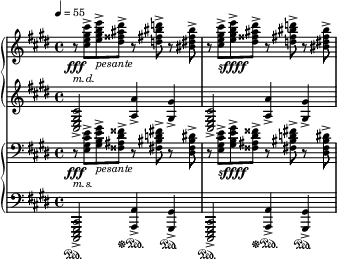
\includegraphics[scale=0.25]{Images/rachm.png}
		\caption{Rachmaninoff Prelude in C Sharp Minor \cite{rm1}}
		\label{rm}
	\end{subfigure}%
	\begin{subfigure}{0.5\textwidth}
		\centering 
		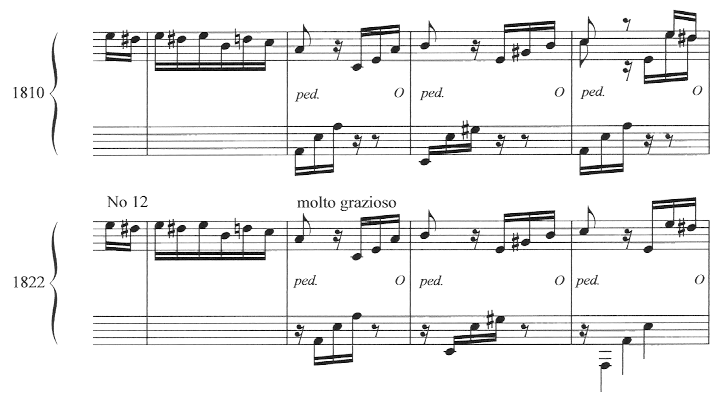
\includegraphics[scale=0.4]{Images/felise.png}
		\caption{Für Elise \cite{fe1}}
		\label{fe}
	\end{subfigure}
	}}
	\caption{Original Scores}
	\label{fig:sheets}
\end{figure}

The first toolkit tested is Aubio \cite{aubio1}. The result can be seen in figure \ref{fea} and figure \ref{raa}
The upper subplot shows the waveform of the first few seconds of each piece. The second plot figures the estimated pitch with green dots. If the pitch is zero, then no pitch could be estimated, most likely because the associated frame contains silence. The blue dots resemble the estimated pitches, where the confidence (shown as the blue graph in the third subplot) is above a certain threshold (the orange line).

\begin{figure}[htbp]
	\centering
	\framebox{\parbox{1\textwidth}{ 
	\begin{subfigure}{0.5\textwidth}
		\centering      
		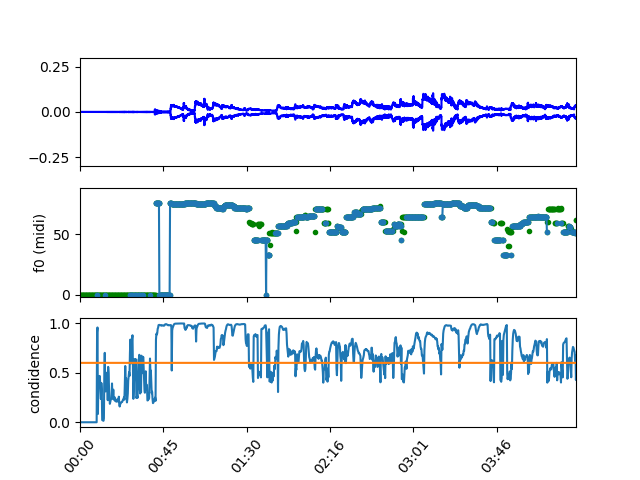
\includegraphics[scale=0.4]{Images/feliseaubio.png}
		\caption{Für Elise Aubio Pitch}
		\label{fea}
	\end{subfigure}%
	\begin{subfigure}{0.5\textwidth}
		\centering 
		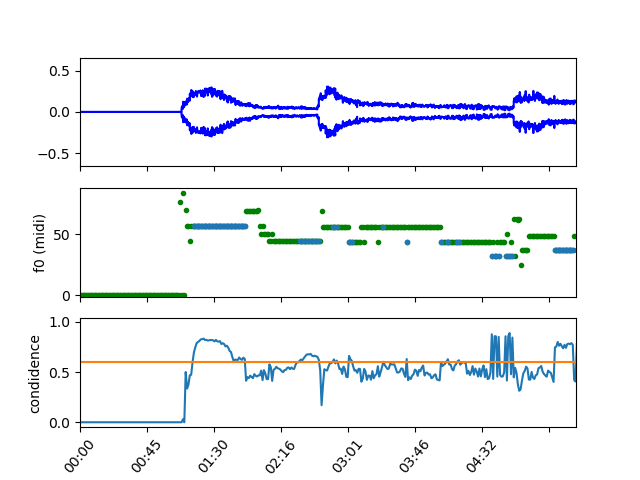
\includegraphics[scale=0.4]{Images/rachaubio.png}
		\caption{Rachmaninoff Prelude Aubio Pitch}
		\label{raa}
	\end{subfigure}
	}}
	\caption{Aubio}
	\label{fig:aubio}
\end{figure}
\FloatBarrier

The other melody extraction tool is Melodia\cite{melodia1}, which is available as a VAMP plugin and can be used together with the Sonic Visualizer\cite{sonviz1}\\
The results are shown in figure \ref{fem} and \ref{ram}.
The purple line is the estimated pitch, however there are large jumps between different octaves of the harmonics. 

\begin{figure}[htbp]
	\centering
	\framebox{\parbox{1\textwidth}{ 
	\begin{subfigure}{0.5\textwidth}
		\centering      
		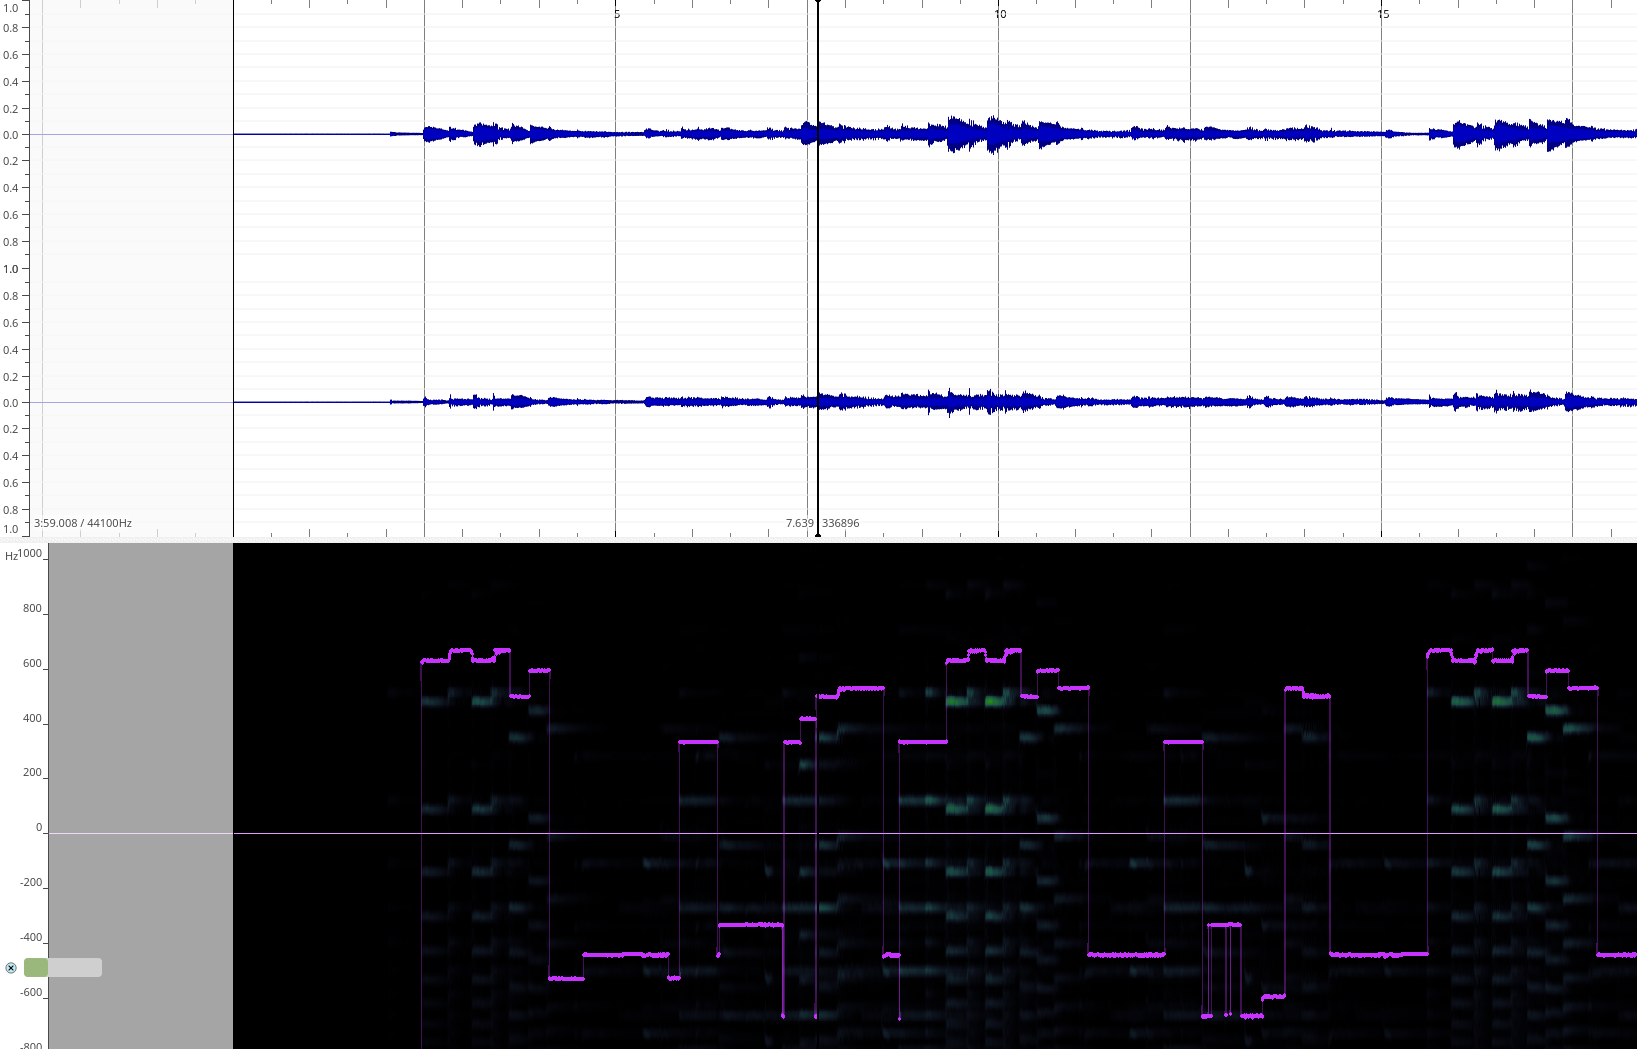
\includegraphics[scale=0.13]{Images/femelodia.png}
		\caption{Für Elise Melodia Pitch}
		\label{fem}
	\end{subfigure}%
	\begin{subfigure}{0.5\textwidth}
		\centering 
		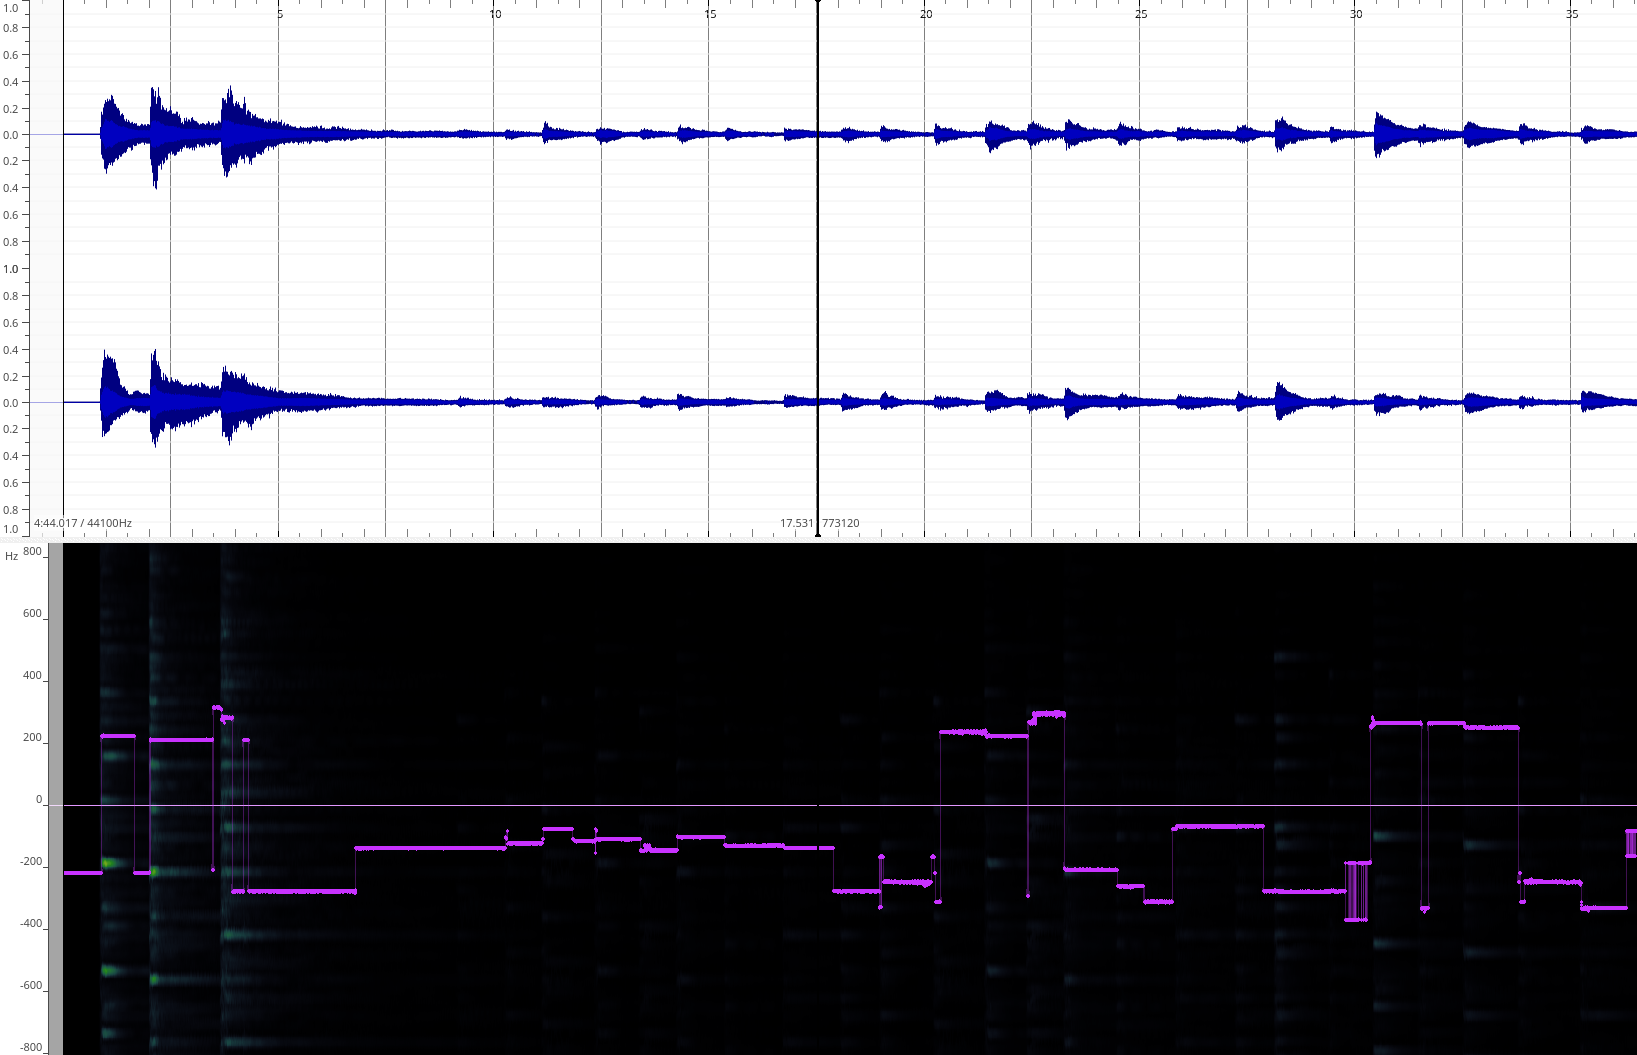
\includegraphics[scale=0.13]{Images/rmmelodia.png}
		\caption{Rachmaninoff Melodia Pitch}
		\label{ram}
	\end{subfigure}
	}}
	\caption{Melodia}
	\label{fig:melodia}
\end{figure}
\FloatBarrier
Sadly the conversion to MIDI does not work flawlessly.\\
Figure \ref{femm} shows the output of a python script using the Melodia VAMP plugin to calculate a MIDI file containing the main melody line.

\begin{figure}[htbp]
	\centering
	\framebox{\parbox{1\textwidth}{ 
	\begin{subfigure}{0.5\textwidth}
		\centering      
		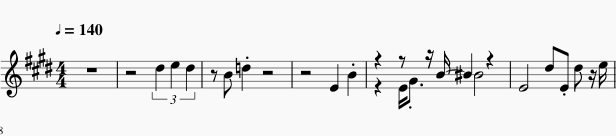
\includegraphics[scale=0.35]{Images/femelodiamidi.png}
		\caption{Für Elise Melodia MIDI}
		\label{femm}
	\end{subfigure}%
	\begin{subfigure}{0.5\textwidth}
		\centering 
		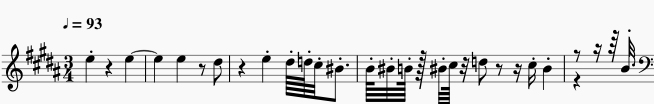
\includegraphics[scale=0.33]{Images/feam.png}
		\caption{Für Elise Aubio MIDI}
		\label{feam}
	\end{subfigure}
	}}
	\caption{Transcription}
	\label{fig:transc}
\end{figure}
\FloatBarrier

Work in progress: A script to convert Aubio Pitch to MIDI and the output shown in figure \ref{feam}

\subsection{Spotify API/ Echonest}\label{spotipy}

Another way of getting music information, audio analysis and metadata is by using the Spotify API\cite{spotifyapi1}
Part of the available audio features comes from the Echo Nest\cite{echonest1}
For each song available in Spotify, there are audiofeatures like loudness, speechiness, liveness, instrumentalness, energy, danceability, acousticness, pitch, rhythm bars etc. 
With a small Python library named Spotipy, the available information can very easily be used and accessed. \cite{spotipy1}\\
In figure \ref{spp} the pitch of the piano piece Für Elise by Beethoven is shown and figure \ref{spp2} shows the beginning of the piece in more detail, including green dots, that resemble estimated bar markings. The blue dots represent the note values of one octave. That means they can resemble a value between zero and eleven with zero representing the key C and 11 is representing a B.
The Spotify API actually returns a value for every single one of the keys per segment, while one segment is a section of samples that are relatively uniform in timbre and harmony. In the plots only the most dominant key per segment is shown. 
The pitch values in one segment are normalized to one by their strongest dimension, so the more evenly distributed the pitch values are and the closer they all get to the value one, the more likely it is, that the sample contains only noise.
The Downside using the Spotify API is, that there is no packed and ready to use test dataset containing the relevant features. So for scientific purposes, a test dataset would have to be created first. 

\begin{figure}[htbp]
	\centering
	\framebox{\parbox{1\textwidth}{ 
	\begin{subfigure}{0.5\textwidth}
		\centering      
		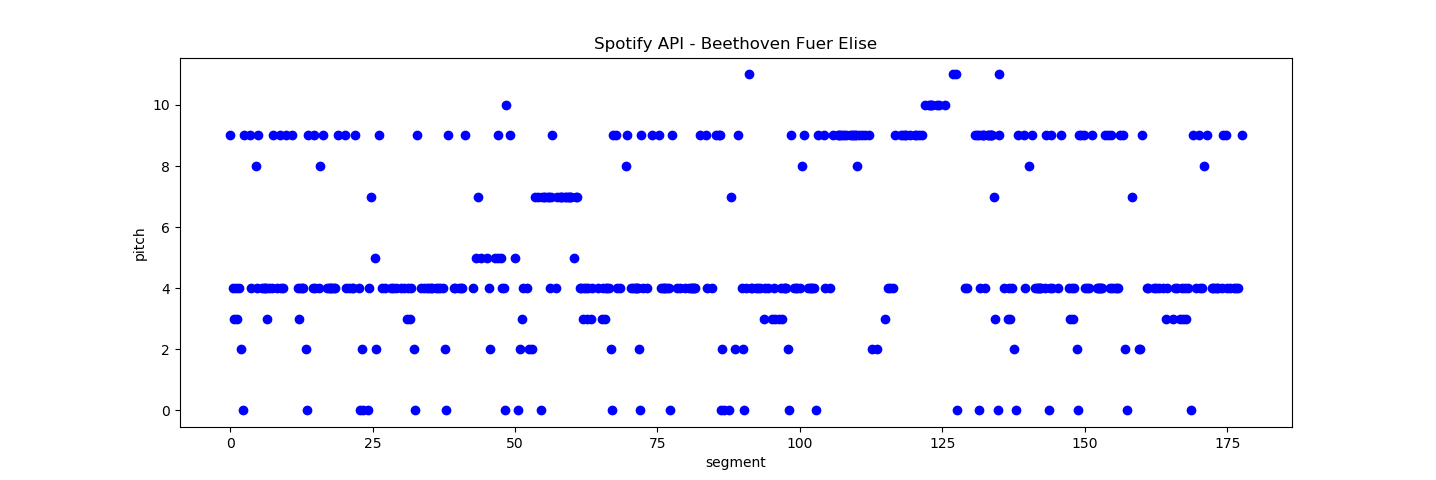
\includegraphics[scale=0.22]{Images/spot1.png}
		\caption{Für Elise Spotify pitch}
		\label{spp}
	\end{subfigure}%
	\begin{subfigure}{0.5\textwidth}
		\centering 
		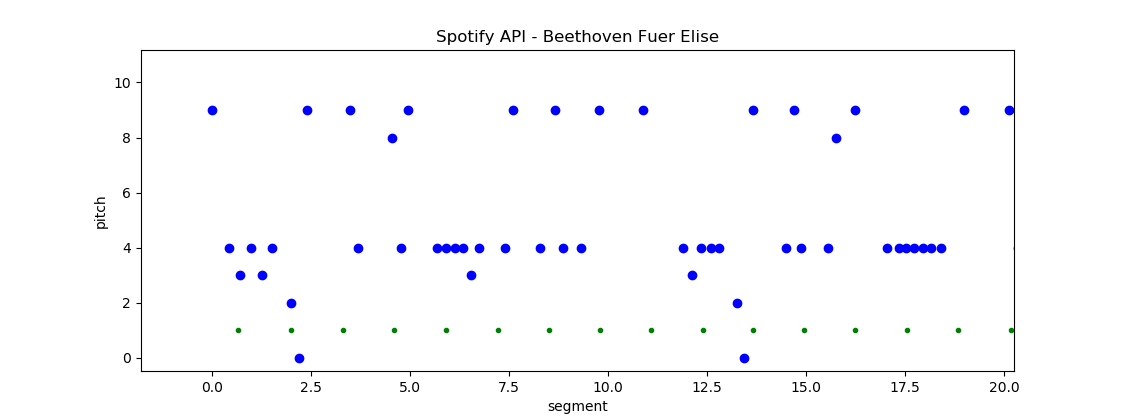
\includegraphics[scale=0.28]{Images/spot2.png}
		\caption{Für Elise detail}
		\label{spp2}
	\end{subfigure}
	}}
	\caption{Spotify API}
	\label{fig:spotify}
\end{figure}
\FloatBarrier

The pitch graph has one significant downside, because it is reduced to one octave and thus can not represent the melody of a song to its full extend. 

\FloatBarrier

\subsection{Cover song identification}

The ability to detect cover songs or different versions/ recording of a musical piece could be a good measurement for the efficiency of music similarity algorithms. In the next section one test case is presented, showing, that a MFCC based music similarity algorithm isn't able to detect different recordings of the same piano piece as most similar to each other. 

\chapter{Data aggregation}

To evaluate the music similarity algorithms and metrics a lot of music data is needed.

\section{Datasets}

\subsection{Free Music Archive}

The largest dataset is the Free Music Archive- dataset (fma) consisting of 106733 different songs totalling an amount of nearly one terabyte of music data from all kinds of different music genres.\cite{fma1} There is also a lot of metadata information available for most of the songs.

\begin{figure}[thpb]
	\centering
	\framebox{\parbox{3in}{      
			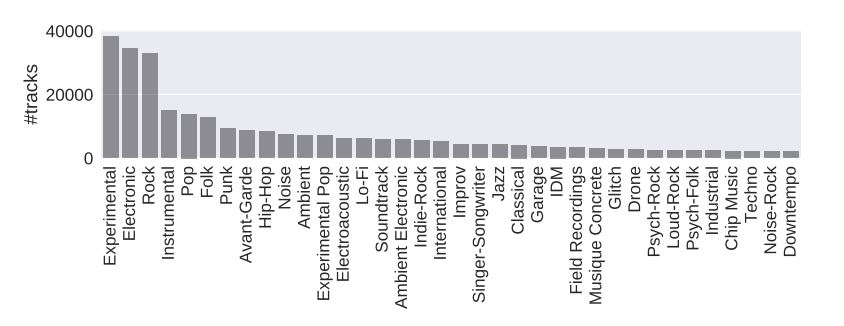
\includegraphics[scale=0.35]{Images/fma_genre.JPG}}}
	\caption{Number of songs in the free music archive dataset per genre}
	\label{fmadist}
\end{figure}
\FloatBarrier

\subsection{Musicnet and 1517 artists}

Another source of music is the Musicnet dataset.\cite{musicnet1} It includes 330 pieces of classical music with musical notes as annotations. 
Other sources of musical information would be the 1517-Artists dataset containing 3180 songs of multiple genres. \cite{1517artists1}

\begin{figure}[thpb]
	\centering
	\framebox{\parbox{3in}{      
			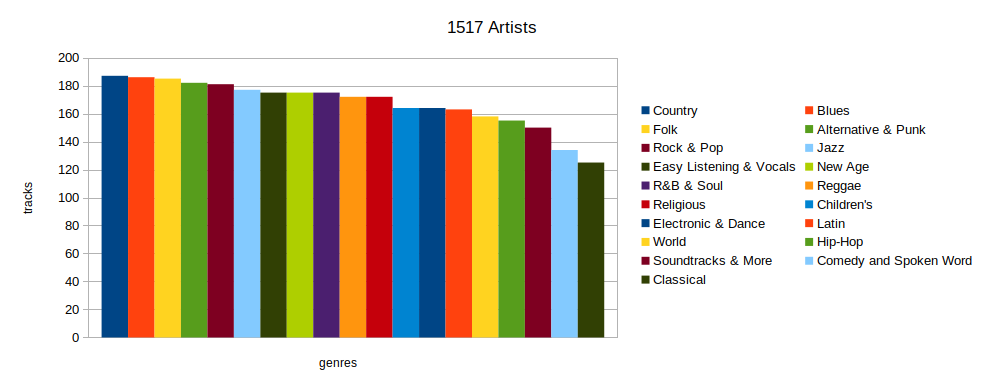
\includegraphics[scale=0.29]{Images/1517genre.png}}}
	\caption{Number of songs in the 1517 artists dataset per genre}
	\label{1517dist}
\end{figure}
\FloatBarrier

\subsection{MedleyDB}

For a melody/ pitch based similarity analysis, multitrack datasets could provide useful data, due to the fact that the pitch estimation can be done instrument by instrument. 
Datasets available are the MedleyDB\cite{medleydb1} and MedleyDB2\cite{medleydb2} datasets as well as the Open Multitrack Dataset\cite{openmult1} currently consisting of 593 multi-tracks in which the MedleyDB dataset is already included, leaving 481 other tracks for analysis.

\begin{figure}[thpb]
	\centering
	\framebox{\parbox{3in}{      
			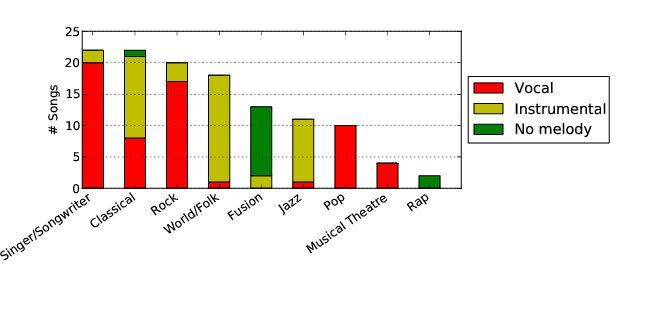
\includegraphics[scale=0.35]{Images/MedleyDB1.png}}}
	\caption{Number of songs in the MedleyDB dataset per genre}
	\label{medleydbdist}
\end{figure}
\FloatBarrier

\subsection{Private music collection}

The private music collection used in this work consist mainly of metal music. The music was legally purchased, all rights belong to the respective owners. The distribution of different songs per genre for this dataset is visualized in figure \ref{privmusdist}.

\begin{figure}[thpb]
	\centering
	\framebox{\parbox{3in}{      
			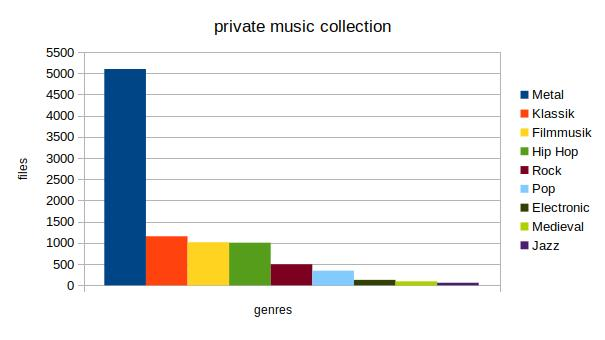
\includegraphics[scale=0.45]{Images/privmus.jpg}}}
	\caption{Number of songs in the private music collection per genre}
	\label{privmusdist}
\end{figure}
\FloatBarrier

Additionally a private recording dataset was used, consisting of ambient recordings and self produced music. Most of this music can be downloaded from soundcloud\cite{bqpd1}
The music sources and amounts of songs used for the task at hand is listed in table \ref{table_dsets}.

\subsection{Overview and other sources}

\begin{table}[h]
	\caption{Music Datasets used}
	\label{table_dsets}
	\begin{center}
		\begin{tabular}{|c||c|}
			\hline
			fma & 106.733 Songs\\
			\hline
			private & 8484 Songs\\
			\hline
			1517 artists & 3180 Songs\\
			\hline
			Maestro & 1184 Songs (piano) + MIDI\\
			\hline
			musicnet & 330 Songs (classical) + note annotation\\
			\hline
			Open Multitrack Testbed & 593(481) Songs/ Multitracks\\
			\hline
			MedleyDB &  122 Songs/ Multitracks\\
			\hline
			MedleyDB2 &  74 Songs/ Multitracks\\
			\hline
		\end{tabular}
	\end{center}
\end{table}

A special and very large dataset is available with the Million Song Dataset (MSD)\cite{msd1}. 
It contains a large set of metadata per track as well as a lot of supplementary datasets, like the Tagtraum genre annotation (figure \ref{msddist})\cite{msd5}, the last.fm dataset\cite{msd2} and the Echo Nest API dataset\cite{msd3}. Although the MSD does not contain any music files in the first place, 30 second samples can be gathered through simple scripts from 7digital.com.
On top of that the Echo Nest API data already contains a lot of audio features like pitch, loudness, energy and danceability to name just a few.
Another addition is the secondhand dataset, containing a list of cover songs in the million song dataset\cite{msd6}


\begin{figure}[thpb]
	\centering
	\framebox{\parbox{3in}{      
			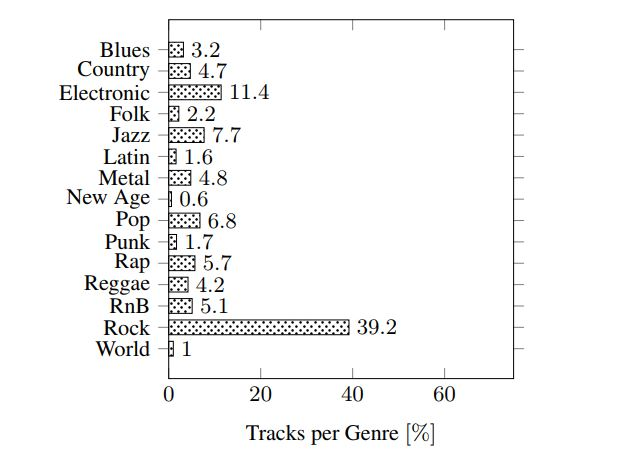
\includegraphics[scale=0.5]{Images/MSD_Tagtraum.JPG}}}
	\caption{Number of songs in the million song dataset per genre}
	\label{msddist}
\end{figure}

Due to the fact that the Spotify API\cite{spotifyapi1} also works with audio features from the Echo Nest\cite{echonest1}, the MSD could be used in a big data environment to simulate the work with Spotify data, without manually mining the actual data.
The MSD was actually already used in Big Data frameworks for music similarity retrieval based on metadata and user information\cite{msd4}\\ 

\section{Spotipy}

For the purpose of this thesis, the option of creating an own dataset using the spotify API and spotipy (section \ref{spotipy}) was considered. 
Ten very small test playlists of different genres were created using the Spotify Playlist Miner \cite{spotmin1}. 
Appendix \ref{spotcrawl} lists a small script, that downloads all audio features and analysis data from all of the songs of a playlist, that contains a preview URL with a 30 second audio snippet.\\
The audio features and analysis data ist saved as a JSON file containing information about (beyond others)

\begin{itemize}
	\setlength\itemsep{0em}
	\item acousticness
	\item danceability
	\item instrumentalness
	\item liveness
	\item loudness
	\item speechiness
	\item valence
	\item predicted key
	\item tempo 
\end{itemize}

as well as pitch and timbre information, beats and bars.\\
\ \\
Together with the 30 second audio sample from which more data like MFCCs could be extracted, these crawler could provide all the information needed to build a large dataset for MIR. However the terms and conditions explicitly prohibits crawling the Spotify service. As stated by the Spotify Terms and Conditions of Use, section 9 (User guidelines):\\
"\textit{The following is not permitted for any reason whatsoever: [...]\\
12. “crawling” the Spotify Service or otherwise using any automated means (including bots, scrapers, and spiders) to view, access, or collect information from Spotify or the Spotify Service;}" \cite{spottac1}\\
Therefore a larger user created dataset can not be used without the risk of legal infringements. However one could argue, that there is a difference between data mining and data crawling and for small datasets with the purpose of creating Spotify playlists, these restrictions may not apply.\\ 
In the sense of the Spotify Developer Terms of Service \cite{spottac2} there may be no legal infringements by creating a non-commercial playlist creation tool. \cite{spottac3} states, that by creating algorithmically-generated playlists similar to the "Discover Weekly" Playlists one may run into challenges if using such features commercially. 
However it does not prohibit the usage for non-commercial cases.  
